\documentclass[10pt]{article}
\usepackage{iftex}
\RequireLuaTeX

\usepackage[hmargin=2.2cm, vmargin=2cm]{geometry}
\usepackage{frenchmath}
\usepackage[dvipsnames,table]{xcolor}
\usepackage{colortbl}
\usepackage{fontspec}
\usepackage{tabularx}
\newcolumntype{C}{>{\centering\arraybackslash}X}
\usepackage{tikz}
\usetikzlibrary{patterns}
\usetikzlibrary{calc}
\usetikzlibrary{math}
\usepackage{amsmath}
\usepackage{scratch3}
\usepackage{wrapfig}
\usepackage{graphicx}

\usepackage[locale=FR, group-digits=all, group-separator=\ , group-minimum-digits=4]{siunitx}
\DeclareSIUnit{\cube}{\cubed}
\DeclareSIUnit{\carre}{\squared}
\DeclareSIUnit{\litre}{\ell}
\usepackage{eurosym}
\DeclareSIUnit{\EURO}{\text{\footnotesize{\euro}}}

\definecolor{Bleu}{HTML}{61A3C9}
\setlength{\parindent}{0pt}

\setsansfont{Archive}[
    Path=../../Polices/Archive/,
    Extension = .otf,
    UprightFont=*
    ]
    
\setromanfont{Marianne}[
    Path=../../Polices/Marianne/,
    Scale=0.8,
    Extension = .otf,
    UprightFont=*-Regular,
    BoldFont=*-Bold,
    ItalicFont=*-RegularItalic,
    BoldItalicFont=*-BoldItalic
    ]
    
\DeclareMathSizes{10}{8}{7}{7} % Pour ajuster la taille des mathématiques et du reste du texte

\pagestyle{empty}
\rmfamily

% Titre du document
\newcommand{\titre}{\sffamily{\huge\color{Bleu}\centerline{ATTENDUS DE FIN D'ANNÉE DE 5\textsuperscript{E}}}\rmfamily}


% Trois symboles
\newcommand{\RR}{
\begin{tikzpicture} \draw[Bleu,fill=Bleu] (0,0) circle (0.06); \end{tikzpicture}}
\newcommand{\LR}{\begin{tikzpicture} \draw[Bleu,fill=Bleu] (0.05,0) -- (0,0.075) -- (-0.05,0) -- (0,-0.075) --cycle; \end{tikzpicture}}
\newcommand{\CR}{\begin{tikzpicture} \draw[Bleu,fill=Bleu] (0,0) -- (0,0.1) -- (0.1,0.1) -- (0.1,0) -- cycle; \end{tikzpicture}}

% Thèmes
\newcommand{\theme}[1]
{\vspace{4ex}\begin{tabularx}{\textwidth}{|XXXX|}\arrayrulecolor{Bleu}
    \multicolumn{4}{c}{\sffamily\color{white}\cellcolor{Bleu}\Large{\phantom{É}#1\phantom{É}}\rmfamily} \\\normalsize
    \RR{} Ce que sait faire l'élève & \LR{} Type d'exercice & \CR{} Exemple d'énoncé & \textit{Indication générale} \\\hline
\end{tabularx}\vspace{3ex}}

% Compétences
\newcommand{\competence}[1]{\par\color{Bleu}\makebox[\linewidth]{\rule{\textwidth}{2pt}}\\{\bfseries\Large#1}\color{black}\vspace{1em}}
\newcommand{\souscompetence}[1]{\par\color{Bleu}\textbf{\large{#1}}\color{black}\vspace{1em}}

% Liste "ce que sait faire l'élève"
\newenvironment{savoireleves}{%
    \renewcommand{\labelitemi}{\RR}%
    \color{black}%
    \par\textbf{Ce que sait faire l'élève}
    \begin{itemize}
    \setlength{\itemsep}{-0.2em}%
}{
    \end{itemize}
}

% Liste "exemples de réussite"
\newenvironment{exemplesreussite}{%
    \renewcommand{\labelitemi}{\LR}%
    \renewcommand{\labelitemii}{-}%
    \color{black}%
    \par\textbf{Exemples de réussite}
    \begin{itemize}
    \setlength{\itemsep}{-0.2em}%
}{
    \end{itemize}
}

\newenvironment{sousitemize}{
    \color{black}%
    \vspace{-1em}%
    \begin{itemize}
    \setlength{\itemsep}{0em}%
}{
    \end{itemize}
}

\newenvironment{sousenumerate}{
    \color{black}%
    \vspace{-1em}%s
    \begin{enumerate}
    \setlength{\itemsep}{0em}%
}{
    \end{enumerate}
}

\begin{document}
    \titre
    \theme{NOMBRES ET CALCULS}
    \competence{Utiliser les nombres pour comparer, calculer et résoudre des problèmes}
    \souscompetence{Nombres}
    
    \begin{savoireleves}
        \item Il utilise, dans le cas des nombres décimaux, les écritures décimales et fractionnaires et passe de l’une à l’autre, en particulier dans le cadre de la résolution de problèmes.
        \item Il relie fractions, proportions et pourcentages.
        \item Il décompose une fraction sous la forme d’une somme (ou d’une différence) d’un entier et d’une fraction.
        \item Il utilise la notion d’opposé.
    \end{savoireleves}
    
    \begin{exemplesreussite}
        \item Il exprime le nombre $2,5+\frac{23}{100} + \frac{7}{5}$ sous formes décimale et fractionnaire.
        \item Pour calculer $20 \%$ de \qty{70}{\EURO}, il effectue $\frac{20}{100} \times 70$ ou $0,2 \times 70$.
        \item Il décompose : $\frac{15}{7} = 2 + \frac{1}{7}$ ou $\frac{15}{7} = 3 - \frac{6}{7}$
        \item Il détermine l’opposé d’un nombre relatif.
        \item Il sait que soustraire revient à additionner l’opposé.
    \end{exemplesreussite}
    
    \souscompetence{Comparaison de nombres}

    \begin{savoireleves}
        \item Il reconnaît et produit des fractions égales.
        \item Il compare, range, encadre des fractions dont les dénominateurs sont égaux ou multiples l’un de l’autre.
        \item Il repère sur une droite graduée les nombres décimaux relatifs.
    \end{savoireleves}

    \begin{exemplesreussite}
        \item[\CR] Dans la liste suivante, entoure toutes les fractions égales à $\frac{14}{6}$ :~~ $\frac{28}{6}$ ; $\frac{7}{3}$ ; $\frac{140}{60}$ ; $\frac{15}{7}$ ; $\frac{15}{7}$ ; $\frac{56}{24}$
        \item Il simplifie $\frac{39}{12}$.
        \item Il range dans l’ordre croissant : $\frac{1}{3}$ ; $\frac{25}{6}$ ; $2$ ; $\frac{5}{3}$.
        \item[\CR] Complète les encadrements suivants par deux entiers consécutifs : $... < \frac{15}{7} < ...$ et $... < \frac{-20}{3} < ...$.
        \item[\CR] Place sur la droite graduée les nombres suivants :\\
        \[ \frac{9}{4}~;~0,25~;~-0.75~;~\frac{5}{4}~;~2,75~;~\frac{5}{2}~;~-1,25 \]
        \begin{center}
        \begin{tikzpicture}[scale=0.5]
            \draw (-9,0) -- (15,0);
            \foreach \x in {-8,-7,...,14} {
                \draw (\x,0.2) -- (\x,-0.2);
            }
            \node[below] at (0,-0.2) {$0$};
            \node[below] at (4,-0.2) {$1$};
        \end{tikzpicture}  
        \end{center}
    \end{exemplesreussite}

    \clearpage
    \competence{Pratiquer le calcul exact ou approché, mental, à la main ou instrumenté}
    \begin{savoireleves}
        \item Il traduit un enchaînement d’opérations à l’aide d’une expression avec des parenthèses.
        \item Il effectue mentalement, à la main ou l’aide d’une calculatrice un enchaînement d’opérations en respectant les priorités opératoires.
        \item Il additionne et soustrait des nombres décimaux relatifs.
        \item Il additionne ou soustrait des fractions dont les dénominateurs sont égaux ou multiples l’un de l’autre.
        \item Il contrôle la vraisemblance d’un résultat.
        \item Il résout des problèmes faisant intervenir des nombres décimaux relatifs et des fractions.
    \end{savoireleves}

    \begin{exemplesreussite}
        \item Pour appliquer le programme de calcul ci-contre au nombre $7$, il effectue le calcul $(7 + 3) \times 9 - 5$.
        \item[\CR] Calcule mentalement : $5 + 3 \times 4$ ; $10 - (1 + 6)$ ; $12 - 8 + 2$.\\
        Calcule à la main : $5,5 + 6 × 2,4$ ; $12 - (5,3 + 3,8)$ ; $16,2 - 9,4 + 3,8$.\\
        Effectue : $(7 + 3) × 9 - 5$.
        \item Il vérifie ses résultats à l’aide de la calculatrice.
        \item[\CR] Calcule mentalement : $-9 + 6$ ; $-5,6 - 3$ ; $4 - 9$ ; $-12 - (-2)$.
        \item Il calcule, sans passer par l’écriture décimale :
        \[ \frac{1}{5} + \frac{2}{5} ; \frac{23}{10} - \frac{5}{10} ; \frac{3}{7} - \frac{2}{7} ; \frac{5}{12} + \frac{4}{3} ; \frac{11}{9} - \frac{1}{3} ; \frac{5}{2} - \frac{1}{4} \]
        \item Il exclut des réponses aberrantes à un problème donné, par exemple \qty{8,12}{\metre} pour la taille d’une personne ou \qty{15}{\centi\metre\carre} pour l’aire d’un champ.
    \end{exemplesreussite}

    \competence{Comprendre et utiliser les notions de divisibilité et de nombres premiers}
    \begin{savoireleves}
        \item Il calcule le quotient et le reste dans une division euclidienne.
        \item Il détermine si un nombre entier est ou n’est pas multiple ou diviseur d’un autre nombre entier.
        \item Il détermine les nombres premiers inférieurs ou égaux à 30.
        \item Il utilise les critères de divisibilité (par $2$, $3$, $5$, $9$, $10$).
        \item Il décompose un nombre entier strictement positif en produit de facteurs premiers inférieurs à $30$.
        \item Il utilise la décomposition en facteurs premiers inférieurs à $30$ pour produire des fractions égales (simplification ou mise au même dénominateur).
        \item Il modélise et résout des problèmes faisant intervenir les notions de multiple, de diviseur, de quotient et de reste.
    \end{savoireleves}

    \begin{exemplesreussite}
        \item[\CR] $147$ élèves sont répartis par équipe de $16$ pour un concours. Combien d’équipes entières peut-on constituer ? Combien manquerait-il d’élèves pour constituer la dernière équipe ?
        \item Il identifie les multiples de 14 parmi les nombres suivants : $56$ ; $141$ ; $280$.
        \item Il dresse la liste des diviseurs de $28$.
        \item Il retrouve la liste des nombres premiers inférieurs à $30$.
        \item[\CR] Détermine, parmi les nombres $2$, $3$, $5$, $9$ et $10$, les diviseurs de $456$ et $1980$.

        \clearpage
        \item Il décompose 84 en produit de facteurs premiers.
        \item Il utilise la décomposition en produit de facteurs premiers pour simplifier $\frac{153}{85}$ .
        \item[] \textit{Problèmes faisant intervenir les notions de multiple, de diviseur, de quotient et de reste}
        \item[\CR] Un garçon de café doit répartir $36$ croissants et $24$ pains au chocolat dans des corbeilles.\\
        Chaque corbeille doit avoir le même contenu. Quelles sont les répartitions possibles ?
        \item[\CR] Un bibliothécaire doit répartir $420$ livres sur des étagères. Chaque étagère doit contenir le même nombre de livres.\\
        Est-ce possible avec $18$ étagères ? Avec $21$ étagères ?
    \end{exemplesreussite}

    \competence{Utiliser le calcul littéral}
    \begin{savoireleves}
        \item Il utilise les notations $2a$ pour $a \times 2$ ou $2 \times a$ et $ab$ pour $a × b$, $a^2$ pour $a \times a$ et $a^3$ pour $a \times a \times a$.
        \item Il utilise la distributivité simple pour réduire une expression littérale de la forme $ax + bx$ où $a$ et $b$ sont des nombres décimaux.
        \item Il produit une expression littérale pour élaborer une formule ou traduire un programme de calcul.
        \item Il utilise une lettre pour traduire des propriétés générales.
        \item Il utilise une lettre pour démontrer une propriété générale.
        \item Il substitue une valeur numérique à une lettre pour :
        \begin{sousitemize}
            \item calculer la valeur d’une expression littérale 
            \item tester, à la main ou de façon instrumentée, si une égalité où figurent une ou deux indéterminées est vraie quand on leur attribue des valeurs numériques 
            \item contrôler son résultat.
        \end{sousitemize}
    \end{savoireleves}

    \begin{exemplesreussite}
        \item Il simplifie l’écriture des expressions suivantes : $5 \times a + 3 \times b$ ~~~~ $x \times y$ ~~~~ $2 \times \ell + 2 \times L$ ~~~~ $2 \times \pi \times r$ ~~~~$\pi \times r \times r$ ~~~~ $c \times c \times c$ ~~~~ $3,2 \times x \times 3 \times x$ ~~~~ $4x \times 2x \times 3x$.
        \item Il réduit des expressions du type : $5,2x + 3,4x$ ~~~~ $2,4x - 2,1x$.
        \item[\CR] Élabore une formule permettant de calculer le nombre de carrés à partir du nombre d’étapes :

        \begin{center}
            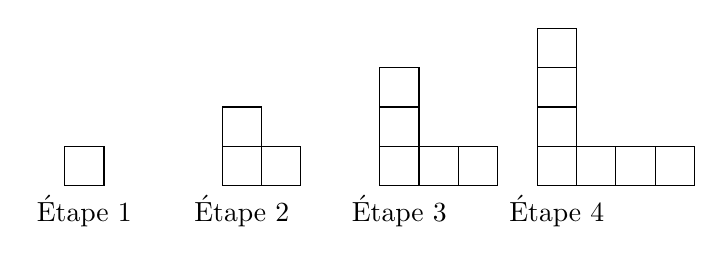
\begin{tikzpicture}[scale=0.5]
                % étape 1
                \coordinate (A) at (0,0);
                \draw ($(A)+(0,0)$) rectangle ($(A)+(0,0)+(1,1)$);
                \node[below] at ($(A)+(0.5,0)$) {Étape $1$};

                % étape 2
                \coordinate (A) at (4,0);
                \draw ($(A)+(0,0)$) rectangle ($(A)+(0,0)+(1,1)$);
                \draw ($(A)+(1,0)$) rectangle ($(A)+(1,0)+(1,1)$);
                \draw ($(A)+(0,1)$) rectangle ($(A)+(0,1)+(1,1)$);
                \node[below] at ($(A)+(0.5,0)$) {Étape $2$};

                % étape 3
                \coordinate (A) at (8,0);
                \draw ($(A)+(0,0)$) rectangle ($(A)+(0,0)+(1,1)$);
                \draw ($(A)+(1,0)$) rectangle ($(A)+(1,0)+(1,1)$);
                \draw ($(A)+(0,1)$) rectangle ($(A)+(0,1)+(1,1)$);
                \draw ($(A)+(2,0)$) rectangle ($(A)+(2,0)+(1,1)$);
                \draw ($(A)+(0,2)$) rectangle ($(A)+(0,2)+(1,1)$);
                \node[below] at ($(A)+(0.5,0)$) {Étape $3$};

                % étape 4
                \coordinate (A) at (12,0);
                \draw ($(A)+(0,0)$) rectangle ($(A)+(0,0)+(1,1)$);
                \draw ($(A)+(1,0)$) rectangle ($(A)+(1,0)+(1,1)$);
                \draw ($(A)+(0,1)$) rectangle ($(A)+(0,1)+(1,1)$);
                \draw ($(A)+(2,0)$) rectangle ($(A)+(2,0)+(1,1)$);
                \draw ($(A)+(0,2)$) rectangle ($(A)+(0,2)+(1,1)$);
                \draw ($(A)+(3,0)$) rectangle ($(A)+(3,0)+(1,1)$);
                \draw ($(A)+(0,3)$) rectangle ($(A)+(0,3)+(1,1)$);
                \node[below] at ($(A)+(0.5,0)$) {Étape $4$};
            \end{tikzpicture}
        \end{center}
        
        \item[\CR] Exprime en fonction du nombre initial le programme de calcul suivant :\\ 
        « Choisir un nombre ; lui ajouter $2$ ; multiplier le résultat par $3$ ; enlever $6$ ».
        \item Il exprime de façon littérale l’entier qui suit un entier $n$, ou l’entier qui le précède.
        \item Il écrit la forme générale d’un multiple de $3$, des nombres entiers naturels pairs et impairs.
        \item Il démontre que la somme de deux entiers consécutifs est impaire.
        \item Il démontre que la somme de trois entiers consécutifs est un multiple de $3$.
        \item Il calcule mentalement $7a$ et $a + 17$ pour $a = 8$.
        \item Il calcule mentalement $3x + 5y$ pour $x = 2$ et $y = 1$.
        \item Il fait un test numérique pour montrer que les expressions $4 + 3x$ et $7x$ ne sont pas égales.
        \item Il utilise une calculatrice pour vérifier ses calculs et ses tests numériques.
    \end{exemplesreussite}

    \clearpage
    \theme{ORGANISATION ET GESTION DE DONNÉES, FONCTIONS}
    \competence{Interpréter, représenter et traiter des données}

    \begin{savoireleves}
        \item Il recueille et organise des données.
        \item Il lit et interprète des données brutes ou présentées sous forme de tableaux, de diagrammes et de graphiques.
        \item Il représente, sur papier ou à l’aide d’un tableur-grapheur, des données sous la forme d’un tableau, d’un diagramme ou d’un graphique.
        \item Il calcule des effectifs et des fréquences.
        \item Il calcule et interprète la moyenne d’une série de données.
    \end{savoireleves}

    \begin{exemplesreussite}
        \item On demande à des élèves leur pointure de pieds ; voici les résultats : 
        \[38 ~~~~ 36 ~~~~ 38 ~~~~ 35 ~~~~ 34 ~~~~ 37 ~~~~ 37 ~~~~ 40 ~~~~ 39 ~~~~ 41 ~~~~ 39 ~~~~ 41 ~~~~ 37 ~~~~ 36 ~~~~ 36 ~~~~ 42 ~~~~ 41 ~~~~ 37 ~~~~ 39 ~~~~ 38. \]
        Complète le tableau suivant :

        \begin{center}
        \begin{tabularx}{0.8\textwidth}{|l|C|C|C|C|C|C|C|C|C|}\hline
            Pointure & 34 & 35 & 36 & 37 & 38 & 39 & 40 & 41 & 42\\\hline
            Effectif & & & & & & & & & \\\hline
        \end{tabularx}
        \end{center}

        \item Il exploite :
        \begin{sousitemize}
            \item un tableau d’effectifs
            \item un diagramme en bâtons
            \item un diagramme circulaire ne faisant pas intervenir des mesures d’angles supérieures à $180$°
            \item un diagramme semi-circulaire
            \item un graphique
        \end{sousitemize}

        \item[] \textit{On demandera de réaliser un diagramme en bâtons, circulaire ou semi-circulaire à partir de données brutes ou d’un tableau d’effectifs.}

        \item Il calcule un effectif total ou la fréquence d’une valeur à partir de données brutes, d’un tableau d’effectifs ou d’un diagramme en bâtons.
        \item[\CR] Complète le tableau suivant qui résume le sport principalement pratiqué par des élèves interrogés au sein d’un collège.

        \begin{center}
        \begin{tabularx}{0.8\textwidth}{|l|C|C|C|C|C|}\hline
            Sport & Football & Tennis & Basket-ball & Athlétisme & \textbf{TOTAL} \\\hline
            Effectif & 26 & 15 & 23 & & \textbf{80} \\\hline
            Fréquence (en \%) & & & & & \\\hline
        \end{tabularx}
        \end{center}

        \item Il sait exprimer des fréquences sous forme fractionnaire, en écriture décimale ou sous la forme d’un pourcentage.
        \item Il calcule une moyenne simple ou pondérée à partir de données brutes, d’un tableau d’effectifs ou d’un diagramme en bâtons.
    \end{exemplesreussite}

    \clearpage
    \competence{Comprendre et utiliser des notions élémentaires de probabilités}
    \begin{savoireleves}
        \item Il place un événement sur une échelle de probabilités.
        \item Il calcule des probabilités dans des situations simples d’équiprobabilité.
    \end{savoireleves} 
    \begin{exemplesreussite}
        \item Il place sur une échelle de probabilité des événements de la vie courante : par exemple obtenir $10$ fois de suite le nombre $6$ en lançant un dé, ne pas gagner la cagnotte du Loto, obtenir pile en lançant une pièce.
        \item Il calcule la probabilité de tomber sur le nombre $2$ en lançant un dé à $6$ faces ; de tomber sur une boule verte en piochant au hasard une boule dans une urne contenant $3$ boules vertes et $4$ boules jaunes.
        \item Il calcule la probabilité de gagner à un jeu (roue de loterie, jeux de dés simples).
    \end{exemplesreussite}

    \competence{Résoudre des problèmes de proportionnalité}
    \begin{savoireleves}
        \item Il reconnaît une situation de proportionnalité ou de non proportionnalité́ entre deux grandeurs.
        \item Il partage une quantité en deux ou trois parts selon un ratio donné.
        \item Il résout des problèmes de proportionnalité dans diverses situations pouvant faire intervenir des pourcentages ou des échelles. Pour cela, il met en œuvre des procédures variées (additivité, homogénéité, passage à l’unité, coefficient de proportionnalité).
    \end{savoireleves}

    \begin{exemplesreussite}
        \item[] \textit{Exemples de situations de proportionnalité : côté et périmètre d’un carré, diamètre et longueur d’un cercle, masse et prix d’une denrée.}
        \item[] \textit{Exemples de non-proportionnalité : côté et aire d’un carré, âge et taille d’une personne.}
        \item Il partage \qty{10}{\EURO} en deux parts selon le ratio $2:3$.
        \item Il retrouve la quantité d’huile et de vinaigre pour \qty{500}{\milli\litre} de vinaigrette réalisée dans le ratio $3:1$.
        \item Il partage une masse de \qty{1,2}{\kilo\gram} en trois parts selon le ratio $1:2:3$ pour une recette de cuisine.
        \item Il applique et calcule des pourcentages simples ($10~\%$ ~;~ $25~\%$ ~;~ $50~\%$) ou des échelles simples ($1:2$ ~;~ $1:4$ ~;~ $1:10$ ~;~...), éventuellement dans le cadre de la résolution de problèmes.
        \item Il calcule une remise pendant les soldes, un prix avant réduction, une distance (réelle, sur une carte).
    \end{exemplesreussite}

    \competence{Comprendre et utiliser la notion de fonction}
    \begin{savoireleves}
        \item Il traduit la relation de dépendance entre deux grandeurs par un tableau de valeur.
        \item Il produit une formule représentant la dépendance de deux grandeurs.
    \end{savoireleves}
    \begin{exemplesreussite}
        \item À partir d’une formule donnée, il traduit dans un tableau de valeurs la dépendance entre la distance de freinage et la vitesse, entre la température ressentie pour un vent de \qty{60}{\kilo\metre\per\hour} et la température ambiante.
        \item Il exprime l’aire d’un carré en fonction de la longueur de son côté, le volume d’un cylindre de rayon \qty{3}{\centi\metre} en fonction de sa hauteur.
    \end{exemplesreussite}

    \clearpage
    \competence{Calculer avec des grandeurs mesurables ; exprimer les résultats dans les unités adaptées}

    \begin{savoireleves}
        \item Il effectue des calculs de durées et d’horaires.
        \item Il calcule le périmètre et l’aire des figures usuelles (rectangle, parallélogramme, triangle, disque).
        \item Il calcule le périmètre et l’aire d’un assemblage de figures.
        \item Il calcule le volume d’un pavé droit, d’un prisme droit, d’un cylindre.
        \item Il calcule le volume d’un assemblage de ces solides.
        \item Il exprime les résultats dans l’unité adaptée.
        \item Il vérifie la cohérence des résultats du point de vue des unités pour les calculs de durées, de longueurs, d’aires ou de volumes.
        \item Il effectue des conversions d’unités de longueurs, d’aires, de volumes et de durées.
        \item Il utilise la correspondance entre les unités de volume et de contenance ($\qty{1}{\litre} = \qty{1}{\deci\metre\cube}$, $\qty{1000}{\litre} = \qty{1}{\metre\cube}$) pour effectuer des conversions.
    \end{savoireleves}

    \begin{exemplesreussite}
        \item Connaissant deux données d’un trajet parmi l’heure de départ, l’heure d’arrivée et la durée, il calcule la donnée manquante. Par exemple, il calcule une heure de départ connaissant la durée du trajet et l’heure d’arrivée.
        \item[\CR] Calcule le périmètre et l’aire de la figure suivante :

        \begin{center}
        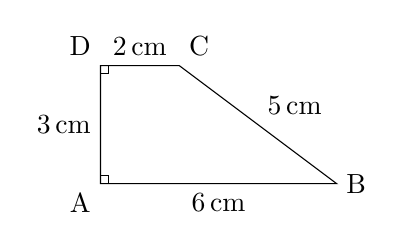
\begin{tikzpicture}[scale=0.5]
            \coordinate (A) at (0,0);
            \coordinate (B) at (6,0);
            \coordinate (C) at (2,3);
            \coordinate (D) at (0,3);
            \draw (A) -- (B) -- (C) -- (D) -- cycle;
            \draw (A) rectangle ($(A)+(0.2,0.2)$);
            \draw (D) rectangle ($(D)+(0.2,-0.2)$);
            \node[anchor=east] at ($(A)!0.5!(D)$) {\qty{3}{\centi\metre}};
            \node[anchor=north] at ($(A)!0.5!(B)$) {\qty{6}{\centi\metre}};
            \node[anchor=south west] at ($(B)!0.5!(C)$) {\qty{5}{\centi\metre}};
            \node[anchor=south] at ($(C)!0.5!(D)$) {\qty{2}{\centi\metre}};
            \foreach \p/\ori in {A/{below left},B/{right},C/{above right},D/{above left}} {
                \node[\ori] at (\p) {\p};
            }
        \end{tikzpicture}
        \end{center}

        \item[\CR] Calcule le volume du solide suivant, composé d’un pavé droit surmonté d’un demi-cylindre (sans considérer le socle) :

        \begin{center}
        \begin{tikzpicture}
            \node[anchor=south west] at (0,0) {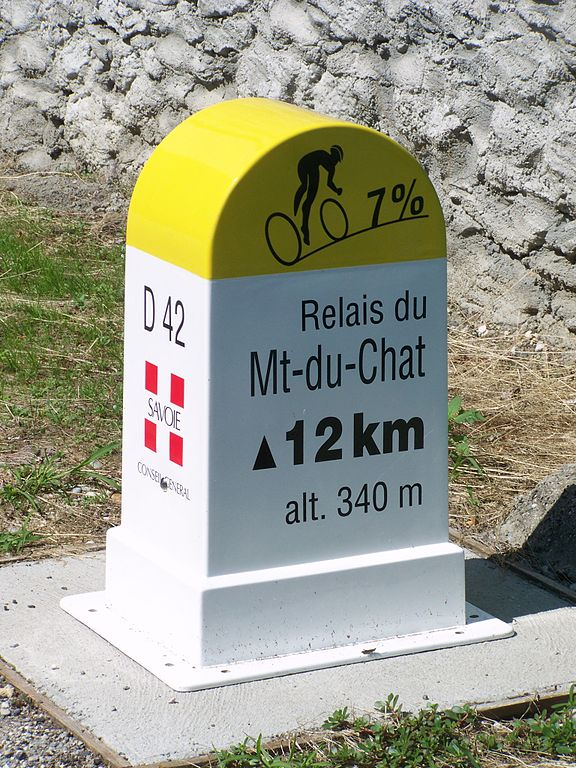
\includegraphics[]{Programmes du B.O./Collège/relais_mont_du_chat_12km.JPG}};
            \draw[latex-latex] (1.19,1.11) -- (0.73,1.39);
            \draw[latex-latex] (1.19,1.11) -- (2.47,1.31);
            \draw[latex-latex] (2.47,1.31) -- (2.47,2.8);
            \node[rotate=-30] at (0.8,1) {\qty{20}{\centi\metre}};
            \node[rotate=10] at (1.9,1) {\qty{40}{\centi\metre}};
            \draw[white,fill=white] (2.58,1.6) rectangle (2.82,2.35);
            \node[rotate=90] at (2.7,2) {\qty{50}{\centi\metre}};
        \end{tikzpicture}
        \end{center}

        \item Il exprime les durées en heures, minutes, secondes, les longueurs en mètres, les aires en mètres carrés et les volumes en mètres cubes.
        \item[\CR] Identifie l’erreur commise dans cette réponse : \\
        « Le volume d’un cube de \qty{3}{\centi\metre} de côté est égal à \qty{27}{\centi\metre\carre}. »
        \item Il convertit \qty{350000}{\metre} en \unit{\kilo\metre} ~~~~ \qty{0.05}{\metre\carre} en \unit{\centi\metre\carre} ~~~~ \qty{12}{\hecto\metre\cube} en \unit{\deci\metre\cube} ~~~~ \qty{2.8}{\hour} en \unit{\hour} et \unit{min}.
        \item Il convertit \qty{33}{\centi\litre} en \unit{\centi\metre\cube} ~~~~ \qty{1500}{\centi\metre\cube} en \unit{\litre}.
    \end{exemplesreussite}

    \clearpage
    \competence{Comprendre l’effet de quelques transformations sur les figures géométriques}

    \begin{savoireleves}
        \item Il comprend l’effet des symétries (axiale et centrale) : conservation du parallélisme, des longueurs et des angles.
        \item Il utilise l’échelle d’une carte.
    \end{savoireleves}

    \begin{exemplesreussite}
        \item Il détermine des longueurs et des mesures d’angles en utilisant les propriétés de conservation des symétries (axiale et centrale).
        \item Il prouve que deux droites sont parallèles en utilisant la conservation du parallélisme par les symétries (axiale et centrale).
        \item Il calcule une longueur en utilisant l’échelle d’une carte.
        \item Il détermine l’échelle d’une carte à partir de longueurs données.
    \end{exemplesreussite}

    \clearpage
    \theme{ESPACE ET GÉOMÉTRIE}
    \competence{Représenter l'espace}

    \begin{savoireleves}
        \item Il se repère sur une droite graduée et dans le plan muni d’un repère orthogonal.
        \item Il reconnaît des solides (pavé droit, cube, cylindre, prisme droit, pyramide, cône, boule) à partir d’un objet réel, d’une image, d’une représentation en perspective cavalière.
        \item Il construit et met en relation une représentation en perspective cavalière et un patron d’un pavé droit, d’un cylindre.
    \end{savoireleves}

    \begin{exemplesreussite}
        \item Il place des points ayant pour coordonnées des nombres relatifs dans un repère orthogonal.
        \item[\CR] Donne les coordonnées des points $A$, $B$ et $C$ placés dans le repère orthogonal suivant. Quelles seraient les coordonnées du point $D$ si on souhaite que $ABCD$ soit un parallélogramme ?

        \begin{center}
        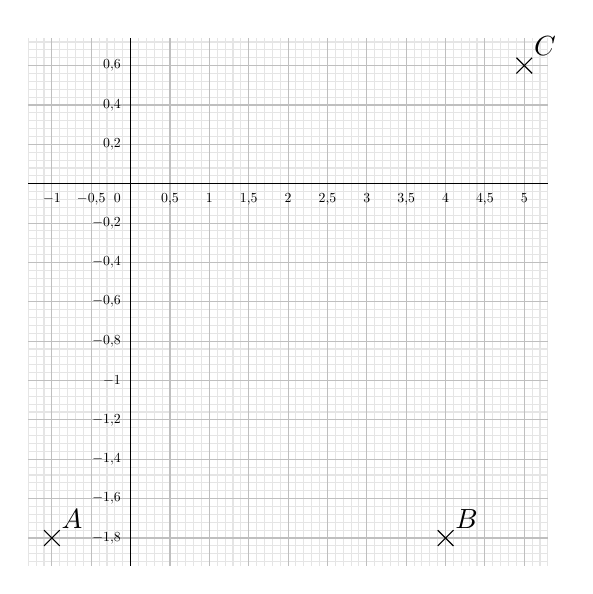
\begin{tikzpicture}[scale=0.5]
            \draw[gray!20!white] (-0.6,-0.7) grid[step=0.2] (12.6,12.7);
            \draw[gray!50!white] (-0.6,-0.7) grid (12.6,12.7);
            \coordinate (A) at (0,0);
            \coordinate (B) at (10,0);
            \coordinate (C) at (12,12);

            \foreach \p in {A,B,C} {
                \tikzmath{\taille = 0.2;}
                \draw ($(\p)+(\taille,\taille)$) -- ($(\p)+(-\taille,-\taille)$);
                \draw ($(\p)+(-\taille,\taille)$) -- ($(\p)+(\taille,-\taille)$);
                \node[above right] at (\p) {$\p$};
            }
            \draw (2,-0.7) -- (2,12.7);
            \draw (-0.6,9) -- (12.6,9);
            \foreach \n/\x in {0/-1,1/-0.5,3/0.5,4/1,5/1.5,6/2,7/2.5,8/3,9/3.5,10/4,11/4.5,12/5} {
                \node[below] at (\n,9) {\scalebox{0.5}{$\num{\x}$}};
            }
            \foreach \n/\y in {0/-1.8,1/-1.6,2/-1.4,3/-1.2,4/-1,5/-0.8,6/-0.6,7/-0.4,8/-0.2,10/0.2,11/0.4,12/0.6} {
                \node[anchor=east] at (2,\n) {\scalebox{0.5}{$\num{\y}$}};
            }
            \node[below left] at (2,9) {\scalebox{0.5}{$0$}};
        \end{tikzpicture}
        \end{center}
        
        \item[\CR] Nomme les solides représentés par les figures suivantes :

        \begin{center}
        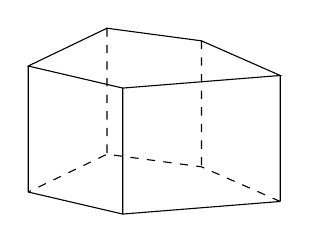
\begin{tikzpicture}[scale=0.4]
            \coordinate (A) at (0.5,-0.2);
            \coordinate (B) at (3.5,-0.9);
            \coordinate (C) at (8.5,-0.5);
            \coordinate (D) at (6,0.6);
            \coordinate (E) at (3,1);
            \coordinate (v) at (0,-4);
            \coordinate (A') at ($(A)+(v)$);
            \coordinate (B') at ($(B)+(v)$);
            \coordinate (C') at ($(C)+(v)$);
            \coordinate (D') at ($(D)+(v)$);
            \coordinate (E') at ($(E)+(v)$);
            \draw (A) -- (B) -- (C) -- (D) -- (E) -- cycle;
            \draw (A') -- (B') -- (C');
            \draw[dashed] (C') -- (D') -- (E') -- (A');
            \draw (A) -- (A') (B) -- (B') (C) -- (C');
            \draw[dashed] (D) -- (D') (E) -- (E');
        \end{tikzpicture}
        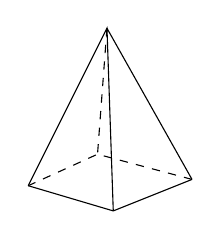
\begin{tikzpicture}[scale=0.4]
            \coordinate (A) at (0.3,0);
            \coordinate (B) at (3,-0.8);
            \coordinate (C) at (5.5,0.2);
            \coordinate (D) at (2.5,1);
            \coordinate (E) at (2.8,5);
            \draw (A) -- (B) -- (C);
            \draw[dashed] (C) -- (D) -- (A);
            \draw (A) -- (E) -- (B) (C) -- (E);
            \draw[dashed] (E) -- (D);
        \end{tikzpicture}
        \end{center}

        \item Il identifie les solides dans des objets du quotidien :

        \begin{center}
            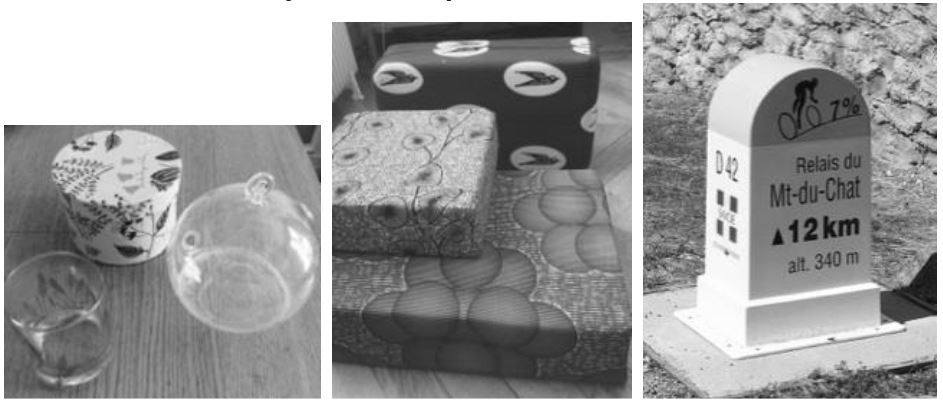
\includegraphics[scale=0.4]{Programmes du B.O./Collège/objets.JPG}
        \end{center}
        \item Il construit la représentation en perspective cavalière d’un cylindre.
        \item Il construit le patron d’un pavé droit.
    \end{exemplesreussite}

    \clearpage
    \competence{Utiliser les notions de géométrie plane pour démontrer}

    \begin{savoireleves}
        \item À partir des connaissances suivantes :
        \begin{sousitemize}
            \item le codage des figures
            \item les caractérisations angulaires du parallélisme (angles alternes internes, angles correspondants)
            \item la somme des angles d’un triangle
            \item l’inégalité triangulaire
            \item une définition et une propriété caractéristique du parallélogramme
            \item la définition de la médiatrice
            \item la définition des hauteurs d’un triangle
        \end{sousitemize}
        il met en œuvre et écrit un protocole de construction de triangles, de parallélogrammes et d’un assemblage de figures.
        \item Il transforme une figure par symétrie centrale.
        \item Il comprend l’effet des symétries (axiale et centrale) sur des figures : conservation du parallélisme, des longueurs et des angles.
        \item Il identifie des symétries dans des frises, des pavages, des rosaces.
        \item Il mobilise les connaissances des figures, des configurations et des symétries pour déterminer des grandeurs géométriques.
        \item Il mène des raisonnements en utilisant des propriétés des figures, des configurations et des symétries
    \end{savoireleves}

    \begin{exemplesreussite}
        \item Il trace des triangles et des parallélogrammes donnés sous forme de figure à main levée ou d’un texte.
        \item[\CR] Trace un triangle $ABC$ isocèle en $B$ tel que $AB = \qty{5}{\centi\metre}$ et $\widehat{ABC} = 130$°.
        \item[\CR] Trace un parallélogramme $GRIS$ tel que $GS = \qty{2}{\centi\metre}$, $SI = \qty{5}{\centi\metre}$ et $\widehat{GSI}$ mesure $50$°.
        \item Il trace en vraie grandeur la figure ci-dessous et explique son protocole de construction.

        \begin{center}
        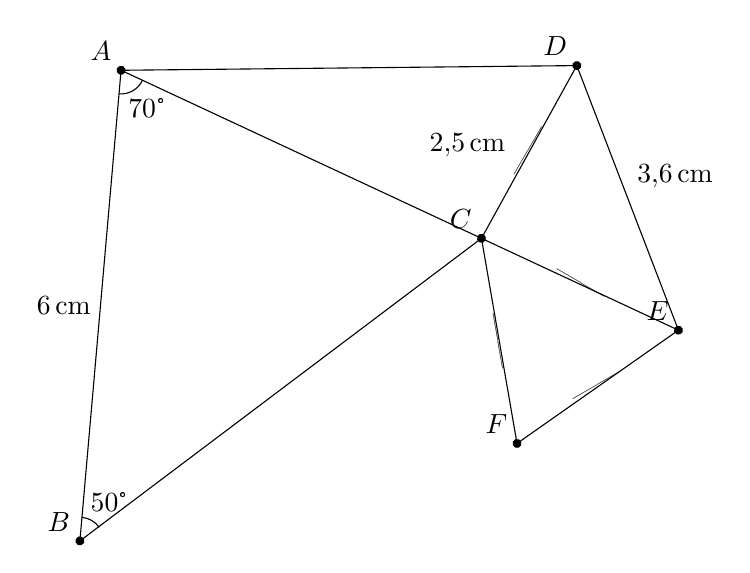
\begin{tikzpicture}[rotate=-25]
            \coordinate (A) at (0,0);
            \coordinate (B) at (2.052,-5.638);
            \coordinate (C) at (5.05,0);
            \coordinate (D) at (5.22,2.5);
            \coordinate (E) at (7.81,0);
            \coordinate (F) at (6.56,-2.17);
            \draw (A) -- (B) -- (C) -- cycle;
            \draw (A) -- (D) -- (C);
            \draw (D) -- (E) -- (F) -- (C) -- (E);

            \foreach \p in {A,B,C,D,E,F} {
                \draw[fill=black] (\p) circle (0.05);
                \node[above left] at (\p) {$\p$};
            }

            \node[anchor=east] at ($(A)!0.5!(B)$) {\qty{6}{\centi\metre}};
            \node[anchor=east] at ($(D)!0.5!(C)+(-0.2,0)$) {\qty{2.5}{\centi\metre}};
            \node[anchor=south west] at ($(D)!0.5!(E)$) {\qty{3.6}{\centi\metre}};
            \node[rotate=60] at ($(C)!0.5!(D)$) {||};
            \node[rotate=-30] at ($(C)!0.5!(E)$) {||};
            \node[rotate=30] at ($(F)!0.5!(E)$) {||};
            \node[rotate=100] at ($(F)!0.5!(C)$) {||};
            \draw (0.3,0) arc (0:-70:0.3);
            \node at (0.5,-0.3) {$70$°};
            \draw ($(B)!0.3cm!(A)$) arc (110:60:0.3);
            \node at ($(B) + (0.13,0.6)$) {$50$°};
        \end{tikzpicture}
        \end{center}
        
        \item Il construit les images par une symétrie centrale de segments, de droites, de cercles, de triangles ou d’assemblages de ces figures.
        \item Il construit en justifiant la démarche et en utilisant plusieurs méthodes le symétrique d’une droite, d’un segment, d’un cercle, d’un triangle par rapport à un point ou à une droite.

        \clearpage

        \item[\CR] Identifie des symétries dans le pavage dont on a représenté une portion ci-dessous :

        \begin{center}
            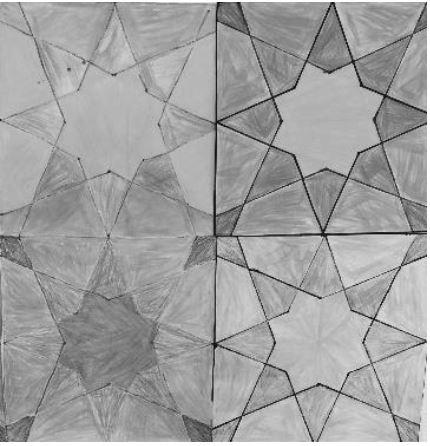
\includegraphics[scale=0.5]{Programmes du B.O./Collège/pavage.jpg}
        \end{center}
        
        \item Il identifie des symétries dans la frise dont on a représenté une portion ci-dessous :

        \begin{center}
        
\begin{tikzpicture}[scale=0.4]
            \coordinate (A) at (0,0);
            \coordinate (v) at (4,0);
            \foreach \n in {0,1,...,7} {
                \draw[fill=gray] ($(A)+\n*(v)$) arc (180:0:1) arc (0:-180:0.5) arc (0:180:0.5);
                \draw[fill=gray] ($(A)+{\n+1}*(v)$) arc (0:180:1) arc (-180:0:0.5) arc (180:0:0.5);
            }
        \end{tikzpicture}
        \end{center}
        
        \item Il détermine l’aire de la portion de frise suivante connaissant l’aire du motif élémentaire « goutte ».

        \begin{center}
        
\begin{tikzpicture}[scale=0.4]
            \coordinate (A) at (0,0);
            \coordinate (v) at (4,0);
            \foreach \n in {0,1,...,7} {
                \draw[fill=gray] ($(A)+\n*(v)$) arc (180:0:1) arc (0:-180:0.5) arc (0:180:0.5);
                \draw[fill=gray] ($(A)+{\n+1}*(v)$) arc (0:180:1) arc (-180:0:0.5) arc (180:0:0.5);
            }
        \end{tikzpicture}
        \end{center}
        
        \item[\CR] Dans la configuration suivante, démontre que $ABCD$ est un parallélogramme.

        \begin{center}
        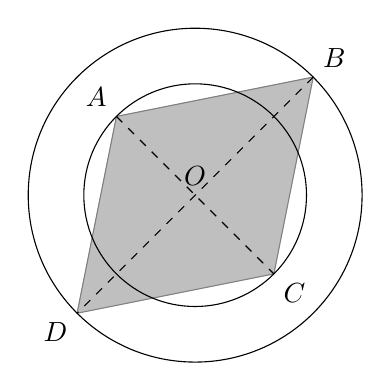
\begin{tikzpicture}
            \coordinate (O) at (0,0);
            \coordinate (A) at (-1,1);
            \coordinate (C) at (1,-1);
            \coordinate (B) at (1.5,1.5);
            \coordinate (D) at (-1.5,-1.5);

            \draw[gray,fill=gray!50!white] (A) -- (B) -- (C) -- (D) -- cycle;
            \draw[dashed] (A) -- (C) (B) -- (D);
            \draw (O) circle (1.414);
            \draw (O) circle (2.12);

            \foreach \p/\ori in {A/{above left},B/{above right},C/{below right},D/{below left},O/above} {
                \node[\ori] at (\p) {$\p$};
            }
        \end{tikzpicture}
        \end{center}
    \end{exemplesreussite}

    \clearpage
    \theme{ALGORITHME ET PROGRAMMATION}
    \centerline{\textbf{\textit{Le niveau 1 est attendu en fin de 5e ; il est possible que certains élèves aillent au-delà.}}}
    \competence{Écrire, mettre au point, exécuter un programme}

    \begin{savoireleves}
        \item[] \textbf{\textit{Niveau $1$}}
        \item Il réalise des activités d’algorithmique débranchée.
        \item Il met en ordre et/ou complète des blocs fournis par le professeur pour construire un programme simple sur un logiciel de programmation.
        \item Il écrit un script de déplacement ou de construction géométrique utilisant des instructions conditionnelles et/ou la boucle « Répéter ... fois ».
        \item[] \textbf{\textit{Niveau $2$}}
        \item Il gère le déclenchement d'un script en réponse à un événement.
        \item Il écrit une séquence d’instructions (condition « si ... alors » et boucle « répéter ... fois »).
        \item Il intègre une variable dans un programme de déplacement, de construction géométrique ou de calcul.
        \item[] \textbf{\textit{Niveau $3$}}
        \item Il décompose un problème en sous-problèmes et traduit un sous-problème en créant un « bloc-personnalisé ».
        \item Il construit une figure en créant un motif et en le reproduisant à l’aide d’une boucle.
        \item Il utilise simultanément les boucles « Répéter ... fois », et « Répéter jusqu’à ... » ainsi que les instructions conditionnelles pour réaliser des figures, des programmes de calculs, des déplacements, des simulations d’expérience aléatoire.
        \item Il écrit plusieurs scripts fonctionnant en parallèle pour gérer des interactions et créer des jeux.
    \end{savoireleves}

    \begin{exemplesreussite}
        \item[] \textbf{\textit{Niveau $1$}}
        \item Il comprend ce que font des assemblages simples de blocs de programmation, par exemple au travers de questions flash.
        \item Il retrouve parmi des programmes donnés celui qui permet d'obtenir une figure donnée, et inversement.
        \item Sans utiliser de langage informatique formalisé, il écrit un algorithme pour décrire un déplacement ou un calcul.
        \item Il décrit ce que fait un assemblage simple de blocs de programmation.
        \item Il ordonne des blocs en fonction d'une consigne donnée.
        \item[\CR] Assemble correctement les blocs ci-contre pour permettre au lutin de tracer un carré de longueur $100$ pixels :

        \begin{center}
        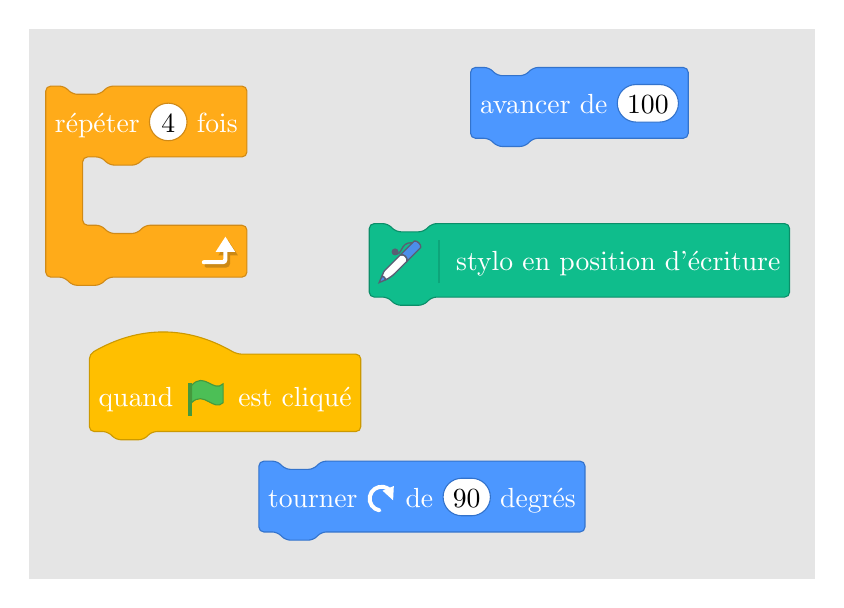
\begin{tikzpicture}
            \draw[white,fill=gray!20!white] (-5,-1) rectangle (5,6);
            \node at (0,0) {\begin{scratch}[pre text=\rmfamily]\blockmove{tourner \turnright{} de \ovalnum{90} degrés}\end{scratch}};
            \node at (-2.5,1.5) {\begin{scratch}[pre text=\rmfamily]\blockinit{quand \greenflag est cliqué}\end{scratch}};
            \node at (2,3) {\begin{scratch}[pre text=\rmfamily]\blockpen{stylo en position d'écriture}\end{scratch}};
            \node at (-3.5,4) {\begin{scratch}[pre text=\rmfamily]\blockrepeat{répéter \ovalnum{4} fois}{\blockspace}\end{scratch}};
            \node at (2,5) {\begin{scratch}[pre text=\rmfamily]\blockmove{avancer de \ovalnum{100}}\end{scratch}};
        \end{tikzpicture}
        \end{center}
        
        \clearpage
        \item[\CR] Il produit seul un programme de construction d’un triangle équilatéral, d’un carré ou d’un rectangle en utilisant la boucle~:
        \begin{center}
        \begin{scratch}[pre text=\rmfamily]
            \blockrepeat{répéter \ovalnum{} fois}{\blockspace}
        \end{scratch}
        \end{center}
        \item[] \textbf{\textit{Niveau $2$}}
        \item Il gère l’interaction entre deux lutins, par exemple en faisant dire une phrase à l’un lorsque l’autre le touche.
        \item Il produit des scripts du type :

        \begin{center}
        \begin{scratch}[pre text=\rmfamily]
            \blockinit{quand \greenflag est cliqué}
            \blockrepeat{répéter \ovalnum{20} fois}{
                \blockvariable{mettre \selectmenu{Nombre aléatoire choisi} à \ovaloperator{nombre aléatoire entre \ovalnum{0} et \ovalnum{1}}}
                \blockif{si \booloperator{\ovalvariable{Nombre aléatoire choisi} = \ovalnum{0}} alors}{
                    \blocklook{dire \ovalnum{Le nombre choisi est 0} pendant \ovalnum{1} secondes}
                }
                \blockif{si \booloperator{\ovalvariable{Nombre aléatoire choisi} = \ovalnum{1}} alors}{
                    \blocklook{dire \ovalnum{Le nombre choisi est 1} pendant \ovalnum{1} secondes}
                }
            }
        \end{scratch}
        \end{center}
        
        \item Il produit seul un programme de construction d’un triangle équilatéral, d’un carré, d’un rectangle ou d’un parallélogramme dans lequel l’utilisateur saisi la mesure de la longueur d’au moins un côté.
        \item[] \textbf{\textit{Niveau $3$}}
        \item Il reproduit une frise donnée reproduisant un motif grâce à un bloc personnalisé.
        \item Il produit un programme réalisant une figure du type :

        \begin{center}
        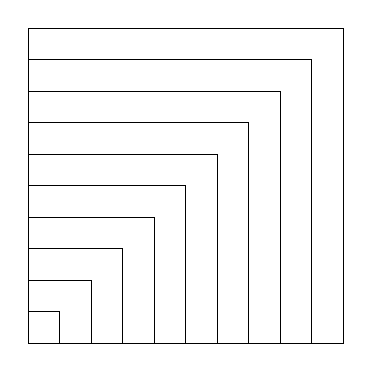
\begin{tikzpicture}[scale=0.4]
            \foreach \n in {1,2,...,9} {
                \draw (\n,0) -- (\n,\n) -- (0,\n);
            }
            \draw (0,0) rectangle (10,10);
        \end{tikzpicture}
        \end{center}
        
        \item Il utilise un logiciel de programmation pour réaliser la simulation d’une expérience aléatoire, par exemple : « Programmer un lutin pour qu’il énonce $100$ nombres aléatoires « $0$ » ou « $1$ » et qu’il compte le nombre de « $0$ » et de « $1$ » obtenus. »
        \item Il programme un jeu avec un logiciel de programmation par blocs utilisant au moins $2$ lutins avec des scripts en parallèle. Il mobilise des capacités acquises précédemment dans les niveaux $1$, $2$ et $3$.
    \end{exemplesreussite}
    
\end{document}